\documentclass[11pt,a4paper]{article}
\usepackage{acl2010}
\usepackage{times}
\usepackage{amsfonts}
\usepackage{subfigure}
\usepackage{amssymb}
\usepackage[small]{caption}
 \usepackage{graphicx}
\usepackage{amsmath}
\usepackage{multirow}
\usepackage{comment}
\usepackage{enumerate}
\usepackage{latexsym}
%\setlength\titlebox{6.5cm}    % Expanding the titlebox

\title{Finding Cognate Groups using Phylogenies}

\author{}

\date{}

\begin{document}
\maketitle
\begin{abstract}
  A central problem in historical linguistics is the identification
  of historically related \emph{cognate} words.  We present a
  phylogenetic model for automatically inducing cognate group
  structure from unaligned word lists.  Our model uses weighted
  transducers to represent distributions over unobserved forms as
  well as the transformations from ancestor word to daughter word.
  We also present a novel method for simplifying the complex automata
  created during inference to counteract the otherwise exponential
  growth of message sizes. We test our model on two datasets where
  we significantly outperform a baseline approach.  Finally, we
  demonstrate that our automatically induced groups can be used to
  successfully reconstruct ancestral words.
\end{abstract}
\section{Introduction}

A crowning achievement of historical linguistics is the comparative
method \cite{ohala93phonetics}, wherein linguists use word similarity
to elucidate the hidden phonological and morphological processes
which govern historical descent. The comparative method requires
reasoning about three important hidden variables: the overall
\emph{phylogenetic guide tree} among languages, the \emph{evolutionary
parameters} of the ambient changes at each branch, and the \emph{cognate
group structure} that specifies which words share common ancestors.

All three of these variables interact and inform each other, and
so historical linguists often consider them jointly.  However,
linguists are currently required to make qualitative judgments
regarding the relative likelihood of certain sound changes, cognate
groups, and so on.  Recent statistical methods have been introduced
to provide increased quantitative backing to the comparative
method~\cite{oakes00computer,bouchard07probabilistic,bouchard09improved}.
These automated methods, while providing robustness and scale in
the induction of ancestral word forms and evolutionary parameters,
assume that both guide trees and cognate words are already given.
In this work, we address the latter, more severe limitation,
presenting a model in which cognate groups can automatically be
discovered.

Finding cognate groups is not an easy task, because underlying
morphological and phonological changes can obscure relationships
between words, especially for distant cognates, where simple string
overlap is an inadequate measure of similarity.  Some authors have
attempted to automatically detect cognate
words~\cite{lowe94reconstruction,oakes00computer,Kondrak01identifyingcognates,mulloni07automatic},
but these methods typically work on language pairs rather than on
language families.  [more?]  To handle realistic scenarios, it is
necessary to consider multiple languages, and to do so in a model
which couples cognate detection with similarity learning.

In this paper we present a new generative model for the automatic
induction of cognate groups given only (1) a known family tree of
languages and (2) word lists from those languages.  A prior on word
survival generates a number of cognate groups and decides which
modern languages attest each group.  An evolutionary model captures
how each word is generated from its parent word.  Finally, a
permutation model describes how cognate groups are collapsed into
flat word lists.  Inference requires a combination of message-passing
in the evolutionary model and iterative bipartite graph matching
in the permutation model.

% This needs to be here to convince latex to put it on page 2. 
\begin{figure*}
  \centering
  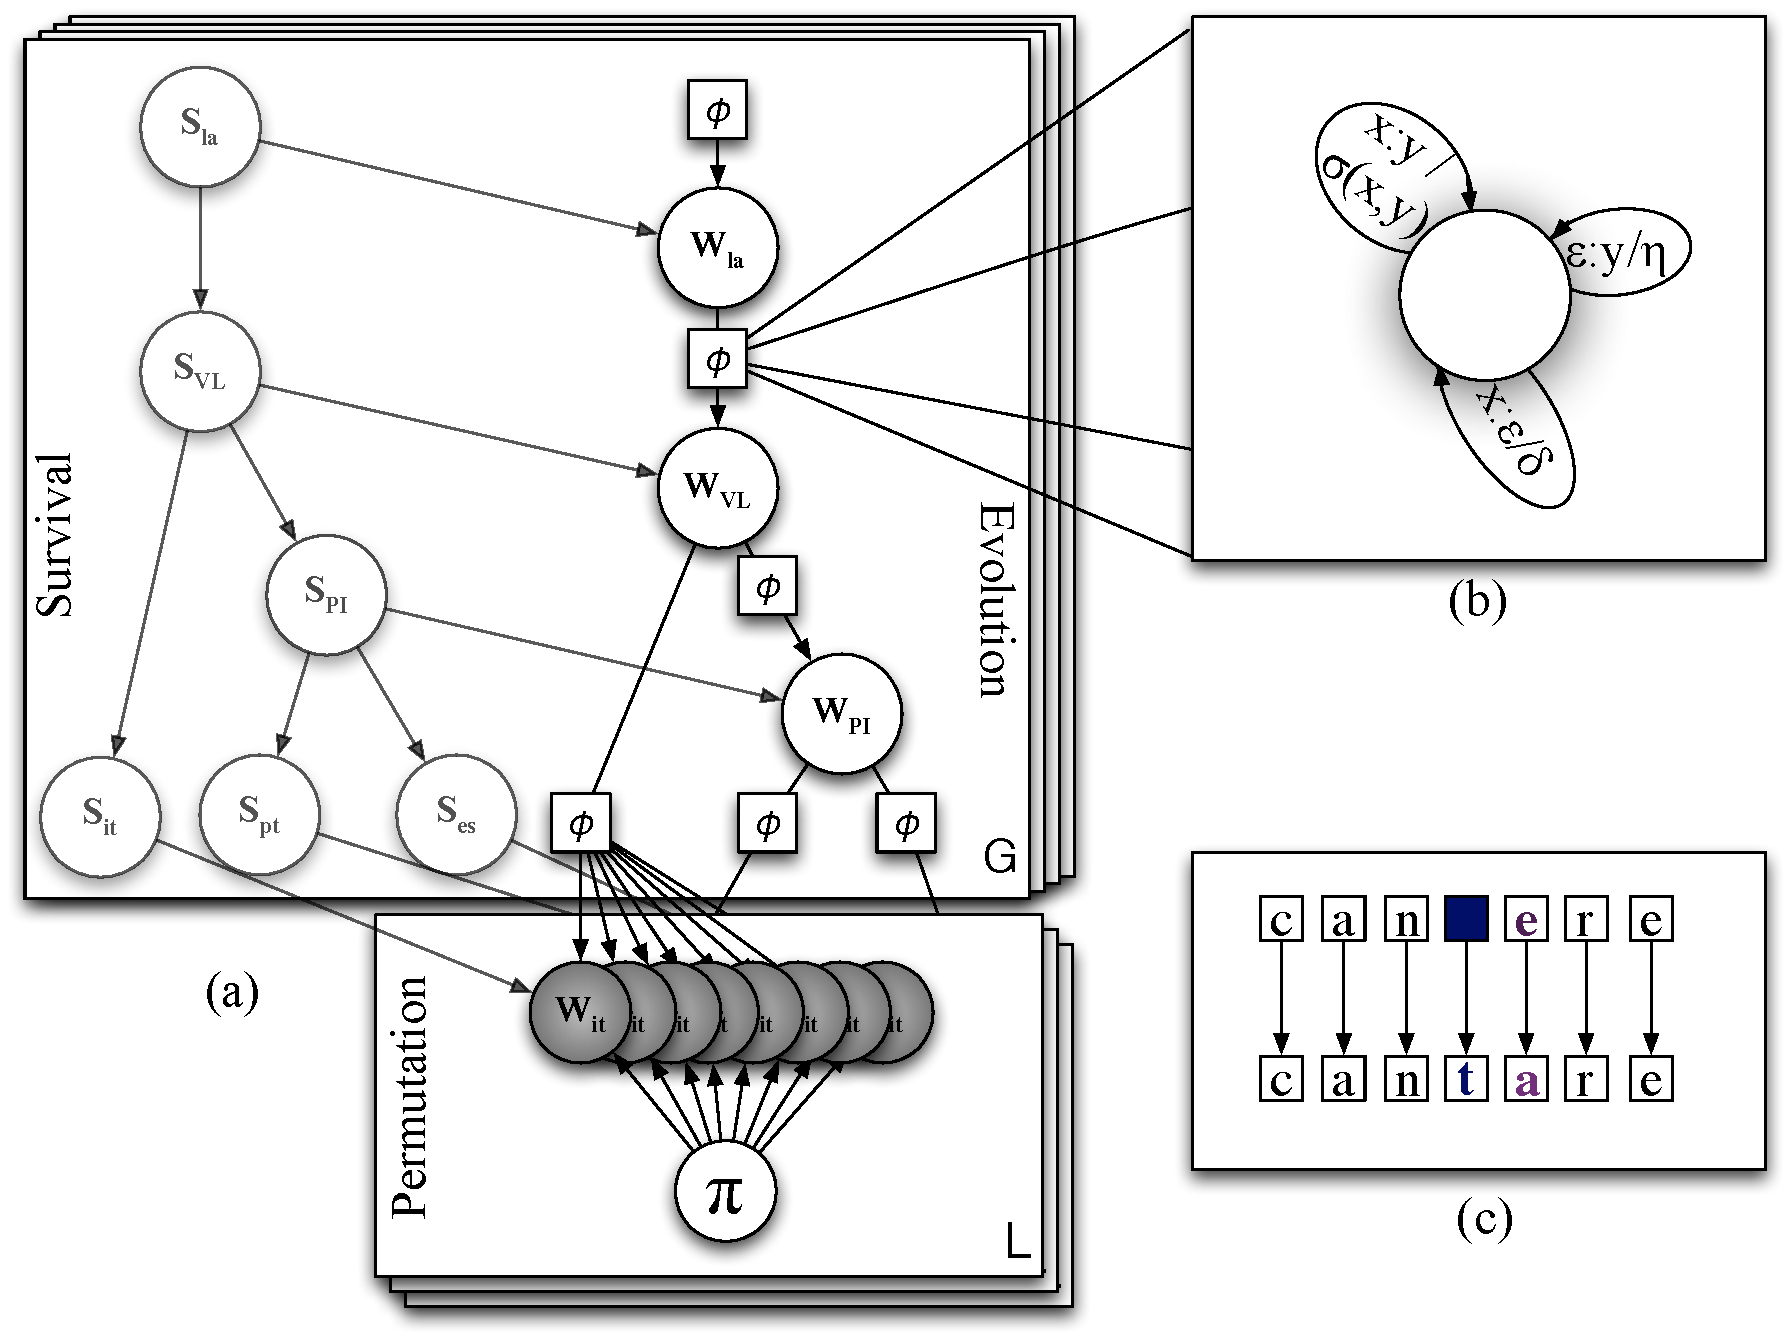
\includegraphics[scale=0.35]{gmodel}
  \caption{(a) The process by which cognate words are generated.
  Here, we show the derivation of Romance language words $W_\ell$
  from their respective Latin ancestor, parameterized by transformations
  $\phi_\ell$ and survival variables $S_\ell$. Languages shown are
  Latin (la), Vulgar Latin (VL), Proto-Iberian (PI), Italian (it),
  Portuguese (pt), and Spanish (es). 
  (b) The class of parameterized edit distances used in this paper.
  Each pair of phonemes has a weight $\sigma$ for deletion, and
  each phoneme has weights $\eta$ and $\delta$ for insertion and
  deletion respectively.
  (c) A possible alignment produced by an edit distance between the
  Latin word \textit{canere} and the Vulgar Latin word \textit{cantare},
  both meaning ``to sing.''} \label{fig:gmodel}
\end{figure*}

In the message-passing phase, our model encodes distributions over
strings as weighted finite state automata~\cite{mohri09weighted}.
Weighted automata have been successfully applied to speech processing
\cite{Mohri96weightedautomata} and more recently to morphology
\cite{dreyer2009graphical}.  Here, we present a new method for
automatically compressing our message automata in a way that can
take into account prior information about the expected outcome of
inference.

%XXX Version 1 (if Romance)

In this paper, we focus on a transcribed word list of 583 cognate
sets from three Romance languages (Portuguese, Italian and Spanish),
as well as their common ancestor Latin~\cite{bouchard07probabilistic}.
We consider both the case where we know that all cognate groups
have a surface form in all languages, and where we do not know that.
On the former, easier, task we achieve accuracies of 90.6\%. On the
latter task, we achieve F1 scores of 72.6. Both easily beat baseline
performance.

\section{Model}

In this section we describe a new generative model for vocabulary lists
in multiple related languages given the phylogenetic relationship
between the languages (their family tree). The generative
process factors into three subprocesses: survival, evolution, and
permutation. Survival dictates, for each cognate group, which
languages have words in that group. Evolution describes the process
by which words are transformed from their parent word. Finally,
permutation describes the ``scrambling'' of the word lists into a flat
order that hides their lineage. Each process is described graphically
in Figure (\ref{fig:gmodel}a) for the Romance languages, and we
present each in detail in the following subsections.

\subsection{Survival}

First, we choose a number of ancestral cognate groups from an
exponential distribution.  For each cognate group, our generative
process walks down the tree.  At each branch, the word may either
survive or die.  This process is modeled in a ``death tree'' with
variables $S_\ell$ specifying whether or not the word died before
reaching that language. Death at any node in the tree causes all
of that node's descendants to also be dead.  This process captures
that a word is more likely to be found in two sibling languages
(e.g. Spanish and Portuguese) than in two cousin languages
(Portuguese and Italian); more independent death events occur in the latter case. 

\subsection{Evolution}

Once we know which languages will have an attested word and which
will not, we generate the actual word forms. The evolution component of
the model generates words according to a branch-specific transformation from a node's 
immediate ancestor.  The figure graphically describes our generative
model for three Romance languages: Italian, Portuguese, and Spanish.
In each cognate group, each word $W_\ell$ is generated from its
parent according to a conditional distribution with parameter $\phi_\ell$,
which is specific to that edge in the tree, but shared between all
cognate groups.

In this paper, each $\phi_\ell$ takes the form of a parameterized
edit distance similar to the standard Levenshtein distance.  Arbitrary
models--such as the richer ones in \newcite{bouchard07probabilistic}--could
instead be used, if at increased inferential cost.   The edit
transducers are represented schematically in Figure (\ref{fig:gmodel}b).
phonemes $x$ and $y$ are arbitrary phonemes, and $\sigma(x,y)$
represents the cost of substituting $x$ with $y$.  $\epsilon$
represents the empty phoneme and is used as short hand for insertion
and deletion, which have parameters $\eta$ and $\delta$, respectively.

As an example, see the illustration in Figure (\ref{fig:gmodel}c).
Here, the Vulgar Latin word \textit{cantare} is generated from its
parent form \textit{canere} by a series of edits: 4 matches, 1
substitution (from `e' to `a') and 1 insertion (`t').
The probability of each individual edit is determined by $\phi$.
Note that the marginal probability of a specific Vulgar Latin word
conditioned on its Latin parent is the sum over all possible
derivations that generate it.

\subsection{Permutation}

Finally, at the leaves of the trees are the observed words. (We
take interior nodes to be unobserved.) Here, we make the (false)
simplifying assumption that in any language there is at most one
word per language per cognate group. Because the assignments of
words to cognates is unknown, we specify an unknown parameter
$\pi_\ell$ for each modern language which is a mapping from cognate
groups to entries in the word list. In the case that every cognate
group has a word in each language, each $\pi_\ell$ is a permutation.
In the more general case that some cognate groups do not have words
from all languages, this mapping is injective from words to cognate
groups. From a generative perspective, $\pi_\ell$ generates observed
positions of the words in some vocabulary list.

In this paper, our task is primarily to learn the permutations
$\pi_\ell$. All other hidden variables are auxiliary and are to be
marginalized to the greatest extent possible.

\section{Inference}
In this section, we discuss the inference method for determining
cognate assignments under fixed parameters $\phi$.  We are given a
set of languages and a list of words in each language, and our
objective is to determine which words are cognate with each other.
In the Romance dataset, we have the additional constraint that each
cognate group supports exactly one word from each language (full
cognate groups), while in the Austronesian dataset we have
at most one word from each language (partial groups). In effect,
the inference task is reduced to finding a permutation $\pi$ of the
respective word lists to maximize the log probability of the observed
words:
\begin{equation}
  \begin{split}
    \vec{\pi} = \arg\!\max_{\vec \pi} \sum_{g} \log p(\vec w_{(\ell,\pi_\ell(g))}|\vec \phi,\vec \pi)
   \end{split}
 \end{equation}
Maximizing this equation directly is intractable, and so instead
we use a coordinate ascent algorithm to iteratively maximize the
permutation corresponding to a single language $\ell$ while holding
the others fixed:
\begin{equation}
  \begin{split}
    \pi_\ell = \arg\!\max_{\pi_\ell} \sum_{g} \log p(\vec w_{(\ell,\pi_\ell(g))}|\vec \phi,\vec \pi_{-\ell},\pi_\ell)
  \end{split}
\end{equation}
Each iteration is then actually an instance of bipartite graph
matching, with the words in one language one set of nodes, and the
current cognate groups in the other languages the other set of
nodes, and the edge affinities $\mathrm{aff}$ between these nodes are the conditional
probability of each word $w_\ell$ belonging to each cognate group $g$:
\begin{equation}
  \begin{split}
    \mathrm{aff}(w_\ell,g) = p(w_\ell|\vec w_{-\ell,\pi_{-\ell}(g)},\vec \phi,\vec\pi_{-\ell})
   \end{split}
 \end{equation}

To compute these affinities for each cognate group, inference in each
tree computes the marginal distribution of the words from the ``held
out'' language. For the marginals, we use an analog of the
forward/backward algorithm. In the upward pass, we send messages
from the leaves of the tree toward the root. For observed leaf nodes
$W_d$, we have:
\begin{equation}
  \begin{split}
    \mu_{d\to a}(w_a) = \sum_{w_d} p(w_d|w_a,\phi)
   \end{split}
 \end{equation}
and for interior nodes $W_i$:
\begin{equation}
  \label{eqn:summing}
  \begin{split}
    \mu_{i\to a}(w_a) = \sum_{w_i} p(w_i|w_a) \prod_{d \in \mathrm{child}(w_i)} \mu_{d \to i}(w_i) 
  \end{split}
\end{equation}
In the downward pass (toward the language $ll$), we sum over ancestral words $W_a$:
\begin{equation}
  \begin{split}
    \mu_{a\to d}(w_d) = \sum_{w_a} p(w_d|w_a) \prod_{\stackrel{d' \in \mathrm{child}(w_a)}{d' \neq d}} \mu_{d' \to a}(w_a) 
  \end{split}
\end{equation}
Computing these messages gives a posterior marginal distribution
$p(w_\ell|\vec w_{-\ell,\pi_{-\ell}(g)},\vec \phi,\vec\pi_{-\ell})$
over the language $ll$, which is precisely the affinity score
we need for the bipartite matching. We then use the Kuhn-Munkres
algorithm \cite{Kuhn1955} to find the optimal assignment for the
bipartite matching problem.

One important final note is initialization. In our early experiments
we found that choosing a random starting configuration unsurprisingly led
to rather poor local optima. Instead, we started with empty trees,
and added in one language per iteration until all languages were
added, and then continued iterations on the full tree.

\section{Learning}

So far we have only addressed searching for Viterbi permutations
$\pi$ under fixed parameters. However, we also have two other sets
of parameters: the transducers $\phi$, and the conditional probabilities
over the survival variables $S_\ell$. The parameters can be learned
through standard maximum likelihood estimation, which we detail in
this section.

Because we enforce that a word must be dead if its parent word is
dead, we just need to learn the conditional probabilities $p(S_\ell|\neg
S_{\mathrm{parent}(\ell)})$ Given fixed assignments $\pi$, we simply
count the number of ``deaths'' that occurred under a live parent,
apply smoothing--we found adding 0.5 to be reasonable--and divide
by the total number of live parents.

For the edit transducers $\phi$, we learn parameterized edit
distances.  For each $\phi_\ell$ we fit a non-uniform substitution,
insertion, and deletion matrix $\sigma(x,y)$. These edit distances
define a conditional exponential family distribution when conditioned
on an ancestral word (or when multiplied by a prior distribution
over those words). That is, for any fixed $w_a$:
\begin{equation*}
  \begin{split}
    \sum_{w_d} &p(w_d|w_a,\sigma) = \sum_{w_d} \sum_{\stackrel{z\in}{\scriptscriptstyle\mathrm{align}(w_a,w_d)}} \mathrm{score}(z;\sigma) \\
    &= \sum_{w_d} \sum_{\stackrel{z\in}{\scriptscriptstyle\mathrm{align}(w_a,w_d)}} \exp( \sum_{(x,y)\in z} \sigma(x,y)) = 1
   \end{split}
 \end{equation*}
where $\mathrm{align}(w_a,w_d)$ is the set of possible alignments between words $w_a$ and $w_d$.

To construct the transducers, we first compute the marginal
distribution over the edges connecting any two languages $a$ and
$d$. With this distribution, we calculate the expected ``alignment
unigrams.'' That is,  for each pair of phonemes $x$ and $y$ (or
empty phoneme $\epsilon$), we need to find the quantity:
\begin{equation*}
  \begin{split}
    E_{p(w_a,w_d)}&[\#(x,y)] \\ = \sum_{w_a,w_d} &\sum_{\stackrel{z\in}{\scriptscriptstyle\mathrm{align}(w_a,w_d)}} \#(x,y;z) p(z|w_a,w_d)p(w_a,w_d)
   \end{split}
 \end{equation*}
where we denote $\#(x,y;z)$ to be the number of times the pair of
phonemes $(x,y)$ are aligned in alignment $z$, and $\#(x,y)$ is the
number of times those phonemes are aligned across all alignments.
The exact method for computing these counts is to use an expectation
semiring~\cite{eisner2001expectation}.

Given the expected counts, we now need to normalize them to ensure
that the transducer represents a conditional probability distribution.
Based on the derivation by \newcite{Oncina20061575}, we have that,
for each phoneme $x$ in the ancestor language:
\begin{equation*}
  \begin{split}
    \sum_{y \in \Sigma \cup \{\epsilon\}} \sigma(x,y) &= 1 - \sum_{y \in \Sigma} \sigma(\epsilon,y) \\
    \sigma(x,y) &\propto \frac{E[\#(x,y)]}{E[\#(x,\cdot)]} \\
    \sigma(\epsilon,y) &= \frac{E[\#(\epsilon,y)]}{E[\#(\cdot,\cdot)]} \\
   \end{split}
 \end{equation*}
Here, $\#(\cdot,\cdot) = \sum_{x,y} \#(x,y)$ and $\#(x,\cdot)=\sum_y
\#(x,y)$. Also, $\sigma(\epsilon,y) = \eta_y$, the insertion
parameter, and $\sigma(x,\epsilon) = \delta_x$, the deletion
parameter.  These equations ensure that the three transition types
(substitution/match, deletion, and insertion) are normalized for
any ancestral phoneme.

\section{Transducers and Approximations}

In our model, it is not just the edit distances that are finite
state machines. Indeed, the words themselves are string-valued
random variables that have, in principle, an infinite domain. To
represent distributions and messages over these variables, we chose
weighted finite state automata, which can compactly represent
functions over strings. Unfortunately, while initially compact,
these automata become unwieldy in inference, and so approximations
must be used~\cite{dreyer2009graphical}.

In this section, we summarize the algorithms and representations
used for weighted finite state transducers.\footnote{For more
detailed treatment of the general transducer operations, we direct
readers to \newcite{mohri09weighted}.} We also describe a new
procedure for approximating automata in a message-passing environment.

\subsection{Weighted Automata}

A weighted automaton (resp. transducer) encodes a function over
strings (resp. pairs of strings) as weighted paths through a directed
graph. Each edge in the graph has a real-valued weight\footnote{The
weights can be anything that form a semiring, but for the sake of
exposition we specialize to real-valued weights} and a label, which
a single phoneme in some alphabet $\Sigma$ or the empty phoneme
$\epsilon$ (resp. pair of labels in some alphabet $\Sigma \times
\Delta$). The weight of a string is then the sum of all paths
through the graph that accept a string.

For our purposes, we are concerned with three fundamental operations
on weighted transducers. The first is computing the sum of all paths
through a transducer, which corresponds to computing the partition
function of a distribution over strings. This operation can be
performed in worst-case cubic time (using a generalization of the
Floyd-Warshall algorithm).  For acyclic or feed-forward transducers
this can be improved dramatically by using a generalization of
Djisktra's algorithm or other related algorithms~\cite{mohri09weighted}.

The second operation is the composition of two transducers.
Intuitively, composition creates a new transducer that takes the
output from the first transducer, processes it through the second
transducer, and then returns the output of the second transducer.
That is, consider two transducers $T_1$ and $T_2$. $T_1$ has input
alphabet $\Sigma$ and output alphabet $\Delta$, while $T_2$ has
input alphabet $\Delta$ and output alphabet $\Omega$. The composition
$T_1 \circ T_2$ returns a new transducer over $\Sigma$ and $\Omega$
such that $(T_1 \circ T_2)(x,y) = \sum_{u} T_1(x,u)\cdot T_2(u,y)$.
In this paper, we use composition for marginalization and factor
products. Given a factor $f_1(x,u;T_1)$ and another factor $f_2(u,y;T_2)$,
composition corresponds to the operation $\psi(x,y) = \sum_u f_1(x,u)
f_2(u,y)$. For two messages $\mu_1(w)$ and $\mu_2(w)$, the same
algorithm can be used to find the product $\mu(w) = \mu_1(w)\mu_2(w)$.

The third operation is transducer minimization. Transducer composition
produces $O(nm)$ states, where $n$ and $m$ are the number of states
in each transducer. Repeated compositions compound the problem:
iterated composition of $k$ transducers produces $O(n^k)$ states.
Minimization alleviates this problem by collapsing indistinguishable
states into a single state. Unfortunately, minimization does not
always collapse enough states. In the next section we discuss approaches
to ``lossy'' minimization that produce automata that are not exactly
the same but are much smaller.

\subsection{Message Approximation}
\label{sec:approx}

Recall that in inference, when summing out interior nodes $w_i$ we
calculated the product over incoming messages $\mu_{d\to i}(w_i)$
(Equation \ref{eqn:summing}), and that these products are calculated
using transducer composition. Unfortunately, the maximal number of
states in a message is exponential in the number of words in the
cognate group. Minimization can only help so much: in order for two
states to be collapsed, the distribution over transitions from those
states must be indistinguishable, or indistinguishable to within
some tolerance. In practice, for the automata generated in our
model, minimization removes at most half the states, which is not
sufficient to counteract the exponential growth. Thus, we need to
find a way to approximate a message $\mu(w)$ using a simpler automata
$\tilde\mu(w;\theta)$ taken from a restricted class parameterized
by $\theta$.

In the context of transducers, previous authors have focused on a
combination of n-best lists and unigram back-off
models~\cite{dreyer2009graphical}.  For their problem, n-best lists
are sensible: their nodes' local potentials already focus messages
on a small number of hypotheses.  In our setting, however, n-best
lists are problematic; early experiments showed that a 10,000-best
list for a typical message only accounts for 50\% of message log
perplexity. That is, the posterior marginals in our model are (at
least initially) fairly flat.

% Put this here to make it come before the section heading Message Topologies
\begin{figure*}
  \centering
  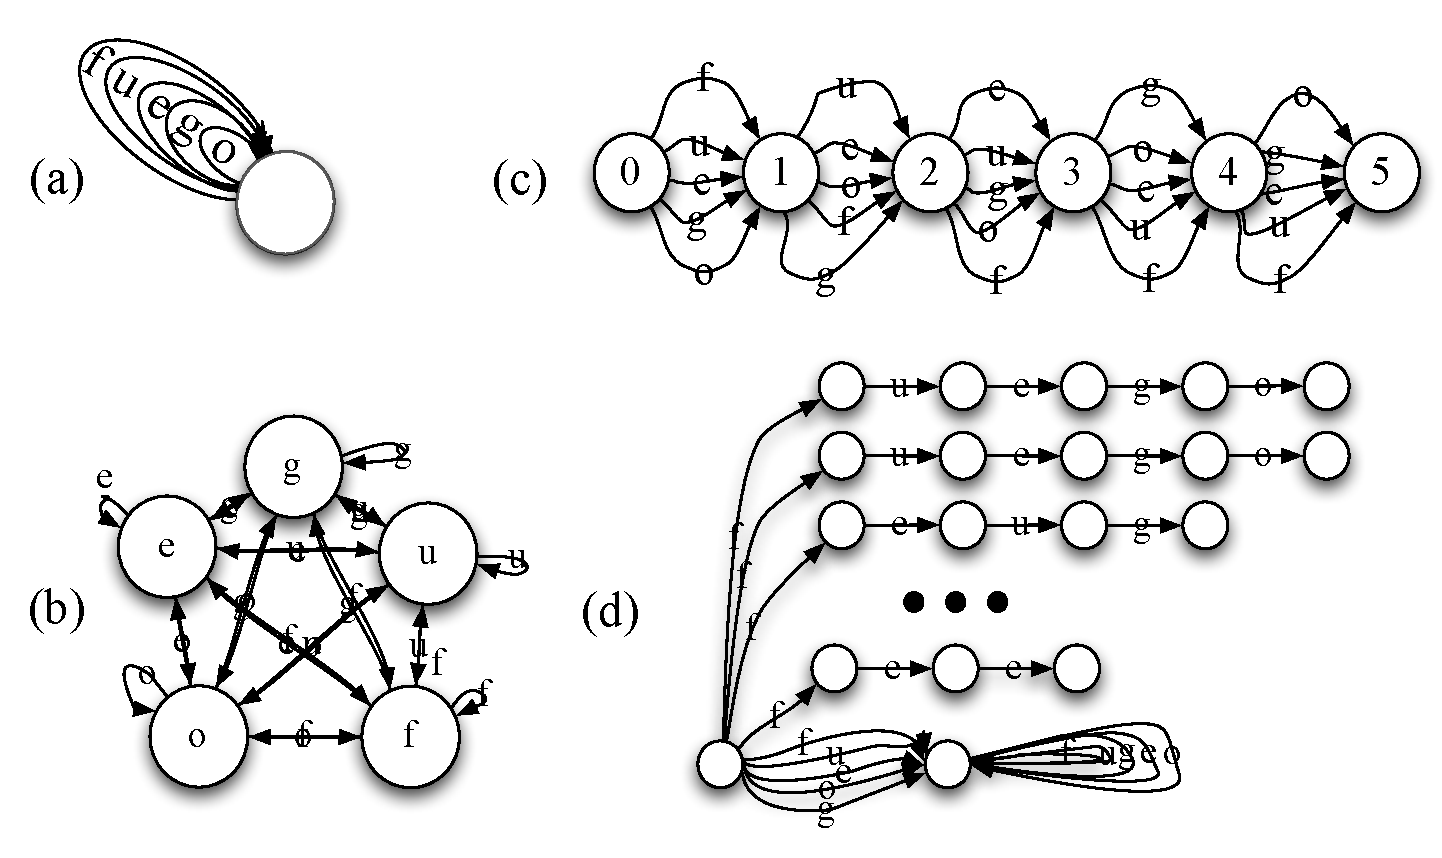
\includegraphics[scale=0.3]{fsa}
  \caption{Various topologies for approximating topologies: (a) a
  unigram model, (b) a bigram model, (c) the anchored unigram model,
  and (d) the n-best plus backoff model used in
  \newcite{dreyer2009graphical}. In (c) and (d), the relative height
  of arcs is meant to convey approximate probabilities.}
  \label{fig:fsa}
\end{figure*}

An alternative approach might be to simply treat messages as
unnormalized probability distributions, and to minimize the KL
divergence between some approximating message $\tilde\mu(w)$ and
the true message $\mu(w)$.  However, messages are not always
probability distributions and--because the number of potential
strings is in principle infinite--they need not sum to a finite
number.\footnote{In an extreme case, suppose we have observed that
$W_d=w_d$ and that $p(W_d=w_d|w_a)=1$ for all ancestral words $w_a$.
Then, clearly $\sum_{w_d} \mu(w_d) = \sum_{w_d} \sum p(W_d=w_d|w_a)
= \infty$ whenever there are an infinite number of possible ancestral
strings $w_a$.} Instead, we propose to minimize the KL divergence
between the ``expected'' marginal distribution and the approximated
``expected'' marginal distribution:
\begin{equation}
  \begin{split}
    \hat\theta &= \arg\!\min_{\theta} D_{KL}(\tau(w)\tilde\mu(w;\theta)||\tau(w)\mu(w) ) \\
    &= \arg\!\min_{\theta} \sum_w \tau(w) \tilde\mu(w;\theta) \log \frac{\tau(w)\tilde\mu(w;\theta)}{\tau(w)\mu(w)} \\
    &= \arg\!\min_{\theta} \sum_w \tau(w) \tilde\mu(w;\theta) \log \frac{\tilde\mu(w;\theta)}{\mu(w)} \\
   \end{split}
 \end{equation}
where $\tau$ is a prior distribution acting as a surrogate for the
posterior distribution over $w$ without the information from $\mu$.
That is, we seek to approximate $\mu$ not on its own, but as it
functions in an environment representing its final context.

In this paper, $\mu(w)$ is a complex automaton with potentially
many states, $\tilde\mu(w)$ is a simple parametric automaton with
forms that we discuss below, and $\tau(w)$ is an arbitrary (but
hopefully fairly simple) automaton. The actual method we use is as
follows. Given a deterministic prior automaton $\tau$, and a
deterministic automaton topology $\tilde\mu^*$, we created the
composed unweighted automaton $\tau \circ \tilde\mu^*$, and calculate
arc transitions weights to minimize the KL divergence between that
composed transducer and $\tau\circ\mu$. The procedure for calculating
these statistics was described in \newcite{li2009first}, which
amounts to using an expectation semiring \cite{eisner2001expectation}
to compute expected transitions in $\tau\circ\tilde\mu^*$ under the
probability distribution $\tau\circ\mu$.

From there, we need to create the automaton $\tau^{-1}
\circ\tau\circ\tilde\mu$. That is, we need to divide out the influence
of $\tau(w)$. Since we know the topology and arc weights for $\tau$
ahead of time, this is often as simple as dividing arc weights in
$\tau\circ\tilde\mu$ by the corresponding arc weight in $\tau(w)$.
For example, if $\tau$ encodes a geometric distribution over word
lengths and a uniform distribution over phonemes (that is, $\tau(w)
\propto {p^{|w|}}$), then computing $\tilde\mu$ is as simple as
dividing each arc in $\tau\circ\tilde\mu$ by $p$.\footnote{Actually,
we must be sure to divide each final weight in the transducer
by $(1-|\Sigma| p)$, which is the stopping probability for a geometric
transducer.}

There are a number of choices for $\tau$. One is a hard maximum on
the length of words. Another is to choose $\tau(w)$ to be a unigram
language model over the language in question with a geometric
probability over lengths. In our experiments, we find that $\tau(w)$
can be a geometric distribution over lengths with a uniform
distribution over phonemes and still obtain reasonable results.
This distribution captures the importance of shorter strings while
still maintaining a relatively weak prior.

\subsection{Message Topologies}

What remains is the selection of the topologies for the approximating
message $\tilde\mu$. We consider three possible approximations,
illustrated in Figure~\ref{fig:fsa}. The first is a plain unigram
model, the second is a bigram model, and the third is an anchored
unigram topology: a position-specific unigram model for each position
up to some maximum length.

The standard unigram model has $|\Sigma|+2$ parameters:
one weight $\sigma_a$ for each phoneme $a \in \Sigma$, a ``starting
weight'' $\lambda$, and a stopping probability. Estimating this
model involves only computing the expected count of each phoneme,
along with the expected length of a word, $E[|w|]$. We then normalize
the counts according to the maximum likelihood estimate, which
gives: 
\begin{equation*}
  \begin{split}
    \sum_{a\in\Sigma} \sigma_a &= \frac{E[|w|]-1}{E[|w|} \\
    \sigma_a &\propto E[\#(a)]
   \end{split}
 \end{equation*}
with the stop probability taking the remaining mass. Recall that
these expectations can be computed using an expectation semiring.

$\lambda$ can be computed by ensuring that the
approximate and exact expected marginals have the same partition
function. That is, with the other parameters fixed solve:
\begin{equation*}
  \begin{split}
    \sum_w \tau(w) \tilde\mu(w) = \sum_w \tau(w) \mu(w)
  \end{split}
\end{equation*}

The second topology we consider is the bigram topology, which is
similar to the unigram topology except that, instead of a single
state, we have a state for each phoneme in $\Sigma$, along with
a special start state. Each state $a$ has transitions with weights
$\sigma_{b|a}= p(b|a) \propto E[\#(b|a)]$. Normalization is similar
to the unigram case, except that we normalize the transitions from
each state.

The final topology we consider takes positional information into
account. Namely, for each position (up to some maximum position),
we have a unigram model over phonemes emitted at that position,
along with the probability of stopping at that position (i.e. a
``sausage lattice''). Estimating the parameters of this model is
similar, except that the expected counts for the phonemes in the
alphabet are conditioned on their position in the string. With the
expected counts for each position, we normalize each state's final
and outgoing weights. In our experiments, we set the maximum length
to 7 + the length of the longest observed string.

\section{Experiments}

We conduct three experiments. The first is a ``complete data''
experiment, in which we reconstitute the cognate groups from the
Romance data set, where all cognate groups have words in all three
languages.  This task highlights the evolution and permutation
models.  The second is a much harder ``partial data'' experiment,
in which we examine a subset of 10 languages in the Oceanic dataset.
Here, only a small fraction of words appear in any cognate group,
so this task crucially involves the survival model.  The ultimate
purpose of the induced cognate groups is to feed richer evolutionary
models, such as full reconstruction models.  Therefore, we also
consider a proto-word reconstruction experiment.  For this experiment,
using the system of \newcite{bouchard09improved}, we compare the
reconstructions produced from our automatic groups to those produced
from gold cognate groups.

\subsection{Baseline}
\label{sec:baseline}

As a baseline for cognate group detection, we use an iterative
bipartite matching algorithm where instead of conditional likelihoods
for affinities we use Dice's coefficient, defined for sets X and
Y as:
\begin{equation}
  \begin{split}
    \mathrm{Dice}(X,Y) &= \frac{2 |X\cap Y|}{|X| + |Y|}
   \end{split}
 \end{equation}
Dice's coefficients are commonly used in bilingual detection of
cognates~\cite{Kondrak01identifyingcognates,Kondrak03cognatescan}.We
follow prior work and use sets of bigrams within words. In our case,
during bipartite matching the set X is the set of bigrams in the
language $\ell$, and Y is the union of bigrams in the other languages.

\subsection{Experiment 1: Complete Data}

In this experiment, we know precisely how many cognate groups there
are and that every cognate group has a word in each language. While
this scenario does not include all of the features of the real-world
task, it represents a good test case of how well these models can
perform without the non-parametric task of decided how many clusters
to use.

We scrambled the 583 cognate groups in the Romance dataset and ran
the algorithm to convergence. Besides the baseline, we tried using
Unigrams, Bigrams and Anchored Unigrams, with and without learning
the parametric edit distances. When we did not use learning, we set
the parameters of the edit distance to (0, -3, -4) for matches,
substitutions, and deletions/insertions, respectively. With learning
enabled, transducers were initialized with these parameters.

For evaluation, we report two metrics. The first is pairwise accuracy
for each pair of languages averaged across pairs. The other is
accuracy measured in terms of the number of correctly and completely
reconstructed cognate groups.

\begin{table}
  \small
  { 
  \begin{tabular}{|c|c|c|c|}
    \hline
    Transducers & Messages & P. Acc. & Rec. Acc. \\
    \hline
    N/A & Baseline & 48.1 & 35.4  \\
    \hline
    Levenshtein&Unigrams & 37.2 & 26.2 \\
    Levenshtein&Bigrams & 43.0 & 26.5 \\
    Levenshtein&Anch. Unigrams & 68.6 & 56.8\\
    \hline 
    Learned&Unigrams & 0.1 & 0.0 \\
    Learned&Bigrams & 38.7 & 11.3 \\
    Learned&Anch. Unigrams & \textbf{90.3}  & \textbf{86.6} \\
    \hline
  \end{tabular}
  \caption{Accuracies for reconstructing cognate groups. Levenshtein
  refers to fixed parameter edit distance transducer. Learned refers
  to automatically learned edit distances. ``P.'' means micro-averaged
  pairwise, ``Rec.'' refers to percentage of completely and accurately
  reconstructed groups. For a description of the baseline, see Section \ref{sec:baseline}. }
  \label{tbl:exp1}
 }
\end{table}

Table \ref{tbl:exp1} shows the results under various configurations.
As can easily be seen, the kind of approximation used matters quite
a lot. In this application, positional information is important,
more so than the context of the previous phoneme. Both Unigrams and
Bigrams significantly under-perform the baseline, while Anchored
Unigrams easily outperforms it both with and without learning.

An initially surprising result is that learning actually harms
performance under the unanchored approximations. The explanation
is that these topologies are not sensitive enough to context, and
that the learning procedure ends up flattening the distributions.
In the case of unigrams--which has the least context--learning
reduces performance to chance. However, in the case of positional
unigrams, learning reduces the error rate by more than two-thirds.

\subsection{Experiment 2: Incomplete Data}

\begin{table}
  \small
  { 
  \begin{tabular}{|c|c|c|c|c|}
    \hline
    Transducers & Messages & Prec. & Recall & F1 \\
    \hline
    N/A & Baseline & 53.3 & 38.2 & 44.5 \\
    Levenshtein&Anch. Unigrams & \textbf{95.3} & 31.5 & 47.3\\
    Learned&Anch. Unigrams  & 62.8 & \textbf{84.3} & \textbf{72.9} \\
    \hline
  \end{tabular}
  \caption{Accuracies for reconstructing incomplete groups. Scores
  reported are precision, recall, and F1, micro-averaged over pairs of words.}
  \label{tbl:partial}
 }
\end{table}

As a more realistic scenario, we consider the case where we do not
know that all cognate groups have words in all languages. To test
our model, we randomly pruned 40\% of the words from the Romance
dataset.

Because only Anchored Unigrams performed well in Experiment 1, we
consider only it and the Dice's coefficient baseline. The baseline
needs to be augmented to support the fact that some words may not
appear in all cognate groups. To do this, we thresholded the bipartite
matching process so that if the coefficient fell below some value,
we started a new group for that word. We experimented on 10 value
in the range (0,1) for the baseline's threshold and report on the
one (0.3) that gives the best pairwise micro-averaged F1.

The results are in Table \ref{tbl:partial}. Here again, we see that
the positional unigrams perform much better than the baseline system.
The learned transducers seem to sacrifice precision for the sake
of increased recall. This makes sense because the default edit
distance parameter settings strongly favor exact matches, while the
learned transducer learns more realistic substitution and deletion
matrices.

\subsection{Experiment 3: Reconstructions}

As a final trial, we wanted to see how each automatically found
cognate group faired as compared to the ``true groups'' for actual
reconstruction of proto-words. Our model is not optimized for
faithful reconstruction, and so we used the Ancestry Resampling
system of \newcite{bouchard09improved}. We matched each Latin word
with the best possible cognate group for that word. The process for
the matching was as follows.

For evaluation, we examined the edit distance between the reconstructed
word and the chosen Latin word. As a skyline, we compare to the
accuracy reported in \newcite{bouchard09improved}, which was based
on complete knowledge of the cognate groups. As you can see XXX

\section{Conclusion}

In this paper, we presented a new generative model of word lists
that automatically finds cognate groups from scrambled vocabulary
lists. This model jointly models the origin, propagation, and
evolution of cognate groups from a common root word. Using the new
approximation technique we introduced in this paper, our model can
reduce the error rate by 80\% over a baseline approach.

Future directions for cognate identification include adding in
semantic information and improving the reconstruction components
for joint identification and reconstruction. \newcite{Kondrak03cognatescan}
showed impressive gains on a bilingual cognate identification task
using semantic distances based on English glosses.  Improving the
reconstruction model could focus on using improved edit distance
models (e.g. \newcite{bouchard09improved}), or further improving
the automata approximations used in this paper. Another important
direction is to extract cognates from raw text, which would most
likely require easing the bipartite assumption.

XXX (conclude conclusively)

\bibliographystyle{acl}
\bibliography{refs}


\end{document}
